\chapter{Approximations of volatility options}\label{ch3}

In this section, we apply KM's method to price options under several mean-reverting models.

\section{Approximating options under mean-reverting CEV model}
\label{sec: 3.1}

\subsection{Auxiliary model selection}

\cite{chan_empirical_1992} proposes the mean-reversion constant elasticity of variance(CEV) model, in which volatility follows

$$
    d V_{t}=\left(\alpha+\beta V_{t}\right) d t+\sigma V_{t}^{\gamma} d W_{t}
$$

\noindent when $\beta$ is negative, this model has mean-reverting property. We can rewrite it to be

\begin{equation}\label{mr}
    d V_t=\kappa(m - V_t) d t+\sigma V^{\gamma}_t d W_t
\end{equation}

\noindent where $\kappa$ is the speed of mean-reversion, $m$ is the long-term mean. A natural idea is follow KM's method, using Black-Scholes model as auxiliary model, then apply their method to approximate the volatility option price under mean-reverting CEV model. Denote $L$ and $L^{\text{bs}}$ to be infinitesimal generators of mean-reverting CEV model and Black-Scholes model respectively

$$
\begin{aligned}
    L w&= \frac{\partial w}{\partial t}+\kappa(m - V) \frac{\partial w}{\partial V}+\frac{1}{2} \sigma^{2} V^{2\gamma} \frac{\partial^{2} w}{\partial V^{2}} \\
    L^{\text{bs}} w &= \frac{\partial w}{\partial t}+rV \frac{\partial w}{\partial V}+\frac{1}{2} \sigma^{2} V^2 \frac{\partial^{2} w}{\partial V^{2}}
\end{aligned}
$$

\noindent The mispricing function for using Black-Scholes model is then

$$\delta^{\text{bs}} = (L - L^{\text{bs}}) w^{\text{bs}} = (\kappa - r)V \frac{\partial w^{\text{bs}}}{\partial t} + \kappa m \frac{\partial w^{\text{bs}}}{\partial t} + \sigma^{2} (V - V^{2 \gamma}) \frac{\partial^{2} w^{\text{bs}}}{\partial V^{2}} $$

\noindent with the solution of Black-Scholes model $w^{\text{bs}}$. Note that $\delta^{\text{bs}}$ contains Theta and Gamma of option. Their differences in Black-Scholes model and mean-reverting model determines that we have to use other auxiliary models. Take call option prices under $\gamma=\frac{1}{2}$ in mean-reverting CEV model\eqref{mr} as an example. This model is known as Square Root(SR) Mean-Reverting model proposed by \cite{grunbichler_valuing_1996}(GL). GL also gives an explicit option price formula under this model, we will use it to illustrate our reason more clearly.


\begin{figure}[ht]
    \centering
    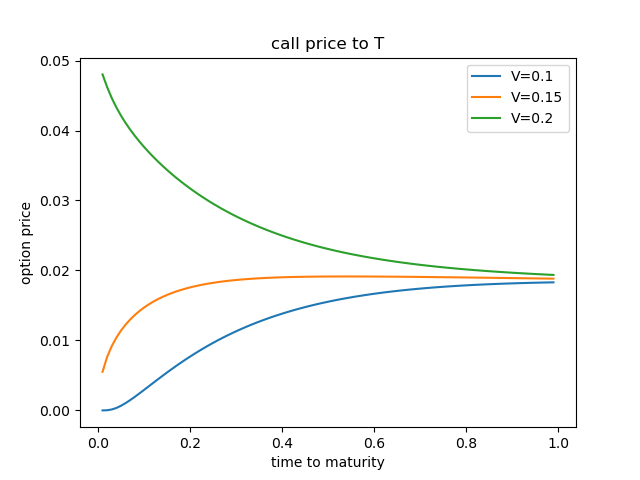
\includegraphics[width=10cm]{./figures/call2T.png}
    \caption{SR mean-reverting call price with regard to time to maturity}\label{call2t}
\end{figure}

\begin{figure}[ht]
    \centering
    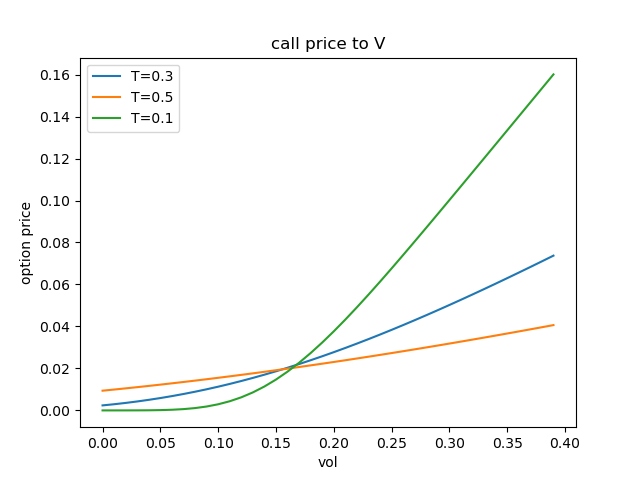
\includegraphics[width=10cm]{./figures/call2V.png}
    \caption{SR mean-reverting call price with regard to volatility}\label{call2v}
\end{figure}

Figure \ref{call2t} and \ref{call2v} are option price changes with the change of time to maturity and underlying asset price correspondingly. From figure \ref{call2t}, we can find that in contrast to Black-Scholes model, the value of call option price under mean-reverting model is not always increasing as time to maturity increases; From figure \ref{call2v}, by contrast, the call option price does not converge to zero like option under Black-Scholes model as volatility goes to zero. In addition, \cite{grunbichler_valuing_1996} also show that $V_t$ has less influence of the current value of the call option than in Black-Scholes model. For these reasons, we conclude that Black-Scholes model is not an appropriate auxiliary model.

Next we discuss that using the SR mean-reverting model as the auxiliary model, it's a special case of mean-reverting CEV model with $\gamma=\frac{1}{2}$

\begin{equation}
    d V_t=\kappa(m - V_t) d t+\sigma \sqrt{V_t} d W_t
\end{equation}

\noindent We are going to use it as our auxiliary model as it captures the mean-reverting property of general mean-reverting CEV models. \cite{grunbichler_valuing_1996} give an explicit option price formula to this model.

\begin{equation}\label{aux call price}
    \begin{aligned}
        \bar{w}=&  e^{ -(\kappa+r) \tau} V Q(x K ; \nu+4, \lambda) \\
        &+ m e^{-r \tau}(1-e^{-\kappa \tau}) Q(xK ; \nu+2, \lambda) \\
        &-e^{-r \tau} K Q(x K; \nu, \lambda)
        \end{aligned}
\end{equation}

\noindent where

$$
\begin{aligned}\label{para}
    & \tau = T-t\\
    &x=\frac{4 \kappa}{\sigma^{2}(1-e^{-\kappa \tau})} \\
    &\nu=\frac{4 \kappa m}{\sigma^{2}}, \\
    &\lambda= e^{-\kappa \tau}x V
    \end{aligned}
$$

\noindent and $Q(xK ; \nu+i, \lambda)$ is the complementary distribution function for the non-central chi-squared density with $\nu + i$ degrees of freedom and non-centrality parameter $\lambda$.

Define the infinitesimal generators $\bar{L}$ for square root mean-reverting model and $L$ for mean-reverting CEV model

\begin{equation}\label{inf gen1}
    \begin{aligned}
        L w&= \frac{\partial w}{\partial t}+\kappa(m - V) \frac{\partial w}{\partial V}+\frac{1}{2} \sigma^{2} V^{2\gamma} \frac{\partial^{2} w}{\partial V^{2}} \\
        \bar{L} w &= \frac{\partial w}{\partial t}+\kappa(m - V) \frac{\partial w}{\partial V}+\frac{1}{2} \sigma^{2} V \frac{\partial^{2} w}{\partial V^{2}}
    \end{aligned}
\end{equation}

Subtract infinitesimal generators in equation\eqref{inf gen1}, we get the mispricing formula for using square root mean-reverting model

$$
\delta = (L - \bar{L}) \bar{w} = \frac{1}{2} \sigma^{2} (V^{2\gamma} - V) \frac{\partial^{2} w}{\partial V^{2}}
$$

\noindent We can then use the approximation formula discussed in \ref{sec: 2.2} to price call options under mean-reverting CEV model\footnote{Put options can be priced easily in the same way}

\begin{equation} \label{cev approx formula}
    w_{N}(t, x)=\bar{w}(t,x)+\sum_{n=0}^{N} \frac{(T-t)^{n+1}}{(n+1) !} \delta_{n}(t, x)
\end{equation}

\noindent where

\begin{equation}\label{mispricing}
    \begin{aligned}
        &\delta_0 = \delta = \frac{1}{2} \sigma^{2} (V^{2\gamma} - V) \frac{\partial^{2} w}{\partial V^{2}} \\
        &\delta_{n}(t, x)=L \delta_{n-1}(t, x)- r\delta_{n-1}(t, x)
        \end{aligned}
\end{equation}

The use of SR mean-reverting model keeps the mean-reverting property in our auxiliary model and provides a simpler mispricing function $\delta(t,x)$. However, call price of SR mean-reverting model, see equation \eqref{aux call price}, contains non-square chi-square distribution functions. Applying infinitesimal generator $L$ on it can be challenging. In the next section we are going to talk about how to derive partial derivatives of distribution function $Q(xK; \nu+i, \lambda)$ with any order.

\subsection{Derivatives of non-central chi-square distribution}

In this section, we introduce our method to calculate derivatives of non-central chi-square distribution and further combine it with approximation methods. Our method is based on the recurrence relation of non-central chi-square distribution proposed by \cite{cohen_noncentral_1988}, which is

\begin{equation}\label{pdf diff}
    \begin{gathered}
        \frac{\partial p(y;\nu,\lambda)}{\partial y}=\frac{1}{2}[-p(y ; \nu, \lambda)+p(y ; \nu-2, \lambda)]\\
        \frac{\partial p(y;\nu,\lambda)}{\partial \lambda}=\frac{1}{2}[-p(y ; \nu, \lambda)+p(y ; \nu+2, \lambda)] \\
    \end{gathered}
\end{equation}

\noindent where $p(y;\nu,\lambda)$ is the Probability Density Function(PDF) of non-central chi-square distribution with degrees of freedom $\nu$ and non-central parameter $\lambda$. From the relationship between Complementary Cumulative Distribution Function(CCDF) $Q(y;\nu,\lambda)$, Cumulative Distribution Function(CDF) $F(y;\nu,\lambda)$, and PDF we know that

\begin{equation}\label{CCDF2x}
    \begin{aligned}
        \frac{\partial Q(y; \nu, \lambda)}{\partial y}&=\frac{\partial[1-F(y; \nu, \lambda)]}{\partial y} \\ 
        &=-\frac{\partial F(y; \nu, \lambda)]}{\partial y}\\
        &= -p(y;\nu,\lambda)
    \end{aligned}
\end{equation}

Combine equation \eqref{pdf diff} and \eqref{CCDF2x} we can derive the derivative of CCDF to non-central parameter $\lambda$. Rewrite the second equation in \eqref{pdf diff}, we get

\begin{equation}\label{pdf trans}
    \begin{aligned}
        \frac{\partial p(y;\nu,\lambda)}{\partial \lambda}&=\frac{1}{2}[-p(y ; \nu, \lambda)+p(y ; \nu+2, \lambda)] \\
        &=-\frac{1}{2}[-p(y ; \nu+2, \lambda)+p(y ; \nu, \lambda)]\\
        &= -\frac{\partial p(y;\nu+2,\lambda)}{\partial y}
    \end{aligned}
\end{equation}

\noindent Integrate both sides of \eqref{pdf trans} with respect to $y$, it's easy to see that

\begin{equation}
    \begin{aligned}
        \frac{\partial}{\partial \lambda} F(y;\nu,\lambda)&=-\frac{\partial}{\partial y}F(y;\nu+2,\lambda) \\
        &= -p(y;\nu+2,\lambda)
    \end{aligned}
\end{equation}

\noindent It's obvious that derivative of CCDF to non-central parameter $\lambda$ is given by

\begin{equation}\label{CCDF2lambda}
    \begin{aligned}
        \frac{\partial Q(y; \nu, \lambda)}{\partial \lambda}&=\frac{\partial[1-F(y; \nu, \lambda)]}{\partial \lambda} \\ 
        &=-\frac{\partial F(y; \nu, \lambda)]}{\partial \lambda}\\
        &= p(y;\nu+2,\lambda)
    \end{aligned}
\end{equation}

Until now we can summarize that the derivatives of CCDF and PDF are all combinations of PDFs with change of degrees of freedom. Without loss of accuracy, we make the degrees of freedom in PDF be similar with call option solution in \eqref{aux call price}, that is for $p(xK;\nu+i, \lambda)$, we let $i \in [2,6]$. Note that in GL's formula degrees of freedom $\nu \in [0,4]$, it we keep the same, it may cause some error when $\nu<2$ in calculating the following derivative

$$
\frac{\partial p(y;\nu,\lambda)}{\partial y}=\frac{1}{2}[-p(y ; \nu, \lambda)+p(y ; \nu-2, \lambda)]
$$

\noindent because degrees of freedom must be larger than 0. Using the non-central chi-square property by \cite{cohen_noncentral_1988} we can do the following transformation to control degrees of freedom in our desired bounds

\begin{equation}\label{trans}
    \begin{aligned}
        p(y ; \nu-2, \lambda)&=\frac{\lambda}{y} p(y ; \nu+2, \lambda)+\frac{v-2}{y} p(y ; \nu, \lambda) \\
        p(y ; \nu+6, \lambda)&=\frac{y}{\lambda} p(y ; \nu+2, \lambda)-\frac{\nu+2}{\lambda} p(y ; \nu+4, \lambda)
    \end{aligned}
\end{equation}

To calculate derivatives of call option price $\bar{w}$ under SR mean-reverting model, we further define some auxiliary derivatives. Recall the parameters $y$, $\nu$ and $\lambda$ in GL's solution \eqref{para}, where

\begin{equation}
    \begin{aligned}
        &y = xK=\frac{4 \kappa}{\sigma^{2}(1-e^{-\kappa \tau})}K \\
        &\nu=\frac{4 \kappa m}{\sigma^{2}}, \\
        &\lambda= e^{-\kappa \tau}x V
    \end{aligned}
\end{equation}

\noindent We define following auxiliary derivatives

\begin{equation}\label{aux diff}
    \begin{aligned}
        \frac{\partial y}{\partial V} &= 0\\
        \frac{\partial \lambda}{\partial V}&= e^{-\kappa \tau}x \\
        \frac{\partial y}{\partial t} &= \frac{-\kappa e^{-\kappa \tau}}{1 - e^{-\kappa \tau}} \cdot xK=\frac{-\kappa e^{-\kappa \tau}}{1 - e^{-\kappa \tau}} y\\
        \frac{\partial \lambda}{\partial t}&= \frac{-\kappa e^{-\kappa \tau}}{1 - e^{-\kappa \tau}} \cdot  xV \\
    \end{aligned}
\end{equation}

Using chain rule, along with these auxiliary derivatives, derivatives of CCDF \eqref{CCDF2x}, \eqref{CCDF2lambda}, derivatives of PDF \eqref{pdf diff}, all partial derivatives related to non-central distribution can be solved as

\begin{equation}\label{ccdf diff2}
    \begin{aligned}
        \frac{\partial Q(y; \nu, \lambda)}{\partial V}=& \frac{\partial Q}{\partial y}\frac{\partial y}{\partial V} + \frac{\partial Q}{\partial \lambda} \frac{\partial \lambda}{\partial V} \\
        =&0 + x e^{-\kappa \tau} p(y ; \nu+2, \lambda)\\
        =& x e^{-\kappa \tau} p(y ; \nu+2, \lambda) \\
        \frac{\partial Q(y; \nu, \lambda)}{\partial t}=& -\frac{\partial Q(y; \nu, \lambda)}{\partial \tau}\\
        =&-\left(\frac{\partial Q}{\partial y}\frac{\partial y}{\partial \tau} + \frac{\partial Q}{\partial \lambda} \frac{\partial \lambda}{\partial \tau}\right) \\
        =& -\frac{-\kappa e^{-\kappa \tau}}{1 - e^{-\kappa \tau}}xK \cdot  [-p(y;\nu,\lambda)]-\frac{-\kappa e^{-\kappa \tau}}{1 - e^{-\kappa \tau}}xV \cdot p(y;\nu+2,\lambda)\\
        =& \frac{\kappa x e^{-\kappa  \tau}}{1 - e^{-\kappa \tau}} \left[-Kp(y;\nu,\lambda) + Vp(y;\nu+2,\lambda)\right]
    \end{aligned}
\end{equation}

and

\begin{equation}\label{pdf diff2}
    \begin{aligned}
        \frac{\partial p(y;\nu,\lambda)}{\partial V} =& \frac{\partial p}{\partial y}\frac{\partial y}{\partial V} + \frac{\partial p}{\partial \lambda} \frac{\partial \lambda}{\partial V} \\
        =& 0+ x e^{-\kappa \tau} \cdot \frac{1}{2} [-p(y; \nu, \lambda)+p(y ; \nu+2, \lambda)]\\
        =& \frac{x e^{-\kappa \tau}}{2} [-p(y ; \nu, \lambda)+p(y ; \nu+2, \lambda)] \\
        \frac{\partial p(y; \nu, \lambda)}{\partial t}=& -\frac{\partial p(y; \nu, \lambda)}{\partial \tau}\\
        =&-\left(\frac{\partial p}{\partial y}\frac{\partial y}{\partial \tau} + \frac{\partial p}{\partial \lambda} \frac{\partial \lambda}{\partial \tau}\right) \\
        =& -\frac{-\kappa e^{-\kappa \tau}}{1 - e^{-\kappa \tau}}xK \cdot  \frac{1}{2}[-p(y ; \nu, \lambda)+p(y ; \nu-2, \lambda)]\\
         &-\frac{-\kappa e^{-\kappa \tau}}{1 - e^{-\kappa \tau}}xV \cdot \frac{1}{2}[-p(y ; \nu, \lambda)+p(y ; \nu+2, \lambda)]\\
        =& \frac{\kappa x e^{-\kappa \tau}}{2(1 - e^{-\kappa \tau})} \left[Vp(y ; \nu+2, \lambda) - (K+V) p(y; \nu, \lambda) + K p(y; \nu-2, \lambda)\right]\\
    \end{aligned}
\end{equation}

Next we use our previous work to calculate Delta

\begin{equation}
    \begin{aligned}
        \Delta_{\bar{w}}=&  e^{ -(\kappa+r) \tau} Q(y ; \nu+4, \lambda) + e^{ -(\kappa+r) \tau}V \cdot x e^{-\kappa \tau} p(y ; \nu+6, \lambda)\\
        &+ m e^{-r \tau}(1-e^{-\kappa \tau}) \cdot x e^{-\kappa \tau} p(y ; \nu+2, \lambda) -e^{-r \tau} K \cdot x e^{-\kappa \tau} p(y ; \nu+2, \lambda)
        \end{aligned}
\end{equation}

\noindent Obviously degrees of freedom in $p(y;\nu+6,\lambda)$ is out of our predefined bounds. We use \eqref{trans} to substitute $p(y;\nu+6,\lambda)$ and simplify the equation

\begin{equation}\label{delta}
    \begin{aligned}
        \Delta_{\bar{w}}=&  e^{ -(\kappa+r) \tau} Q(y ; \nu+4, \lambda) \\
        &+ e^{ -(\kappa+r) \tau} \lambda \left[\frac{y}{\lambda} p(y ; \nu+2, \lambda)-\frac{\nu+2}{\lambda} p(y ; \nu+4, \lambda)\right]\\
        &+ m e^{-r \tau}(1-e^{-\kappa \tau}) \cdot \frac{4 \kappa}{\sigma^{2}(1-e^{-\kappa \tau})} e^{-\kappa \tau} p(y ; \nu+2, \lambda) -e^{-(r+\kappa) \tau} K  p(y ; \nu+2, \lambda) \\
        =& e^{ -(\kappa+r) \tau} [Q(y; \nu+4, \lambda)-2p(y ; \nu+4, \lambda)] 
        \end{aligned}
\end{equation}

Similarly, Gamma of $\bar{w}$ can be calculated by

\begin{equation}\label{gamma}
    \begin{aligned}
        \Gamma_{\bar{w}}&= e^{ -(\kappa+r) \tau} \left[x e^{-\kappa \tau} p(y ; \nu+6, \lambda)-2 \cdot \frac{x e^{-\kappa \tau}}{2} [-p(y ; \nu+4, \lambda)+p(y ; \nu+6, \lambda)]\right] \\
        &= xe^{ -(2\kappa+r) \tau}p(y;\nu+4,\lambda)
    \end{aligned}
\end{equation}

We evaluate our method of calculating partial derivatives by comparing our formula with using finite difference on some range of option prices. Delta, Gamma, Theta calculated by finite difference is given by

$$
\begin{aligned}
    &\Delta^{fm} = \frac{\partial C}{\partial V} \approx \frac{C(V+\Delta)-C(V)}{\Delta V} \\
    &\Gamma^{fm} = \frac{\partial \Delta^{fm}}{\partial V} \approx \frac{\Delta^{fm}(V+\Delta)-\Delta^{fm}(V)}{\Delta V} \\
    &\Theta^{fm} = \frac{\partial C}{\partial t} \approx \frac{C(t+\Delta)-C(t)}{\Delta t} \\
\end{aligned}
$$

\noindent We set step size of finite difference method to be $0.04$, the parameters are $\theta = 0.15, \kappa = 4,\sigma = \sqrt{0.133},r = 0.05, K = 0.15$. $T=0.3$ for Delta and Gamma, $V=0.2$ for Theta. Comparisons are shown in \ref{greeks}, we can find that the result of our method is right and very accurate.

\begin{figure}[ht]
    \centering
    \subfloat[Delta comparison]{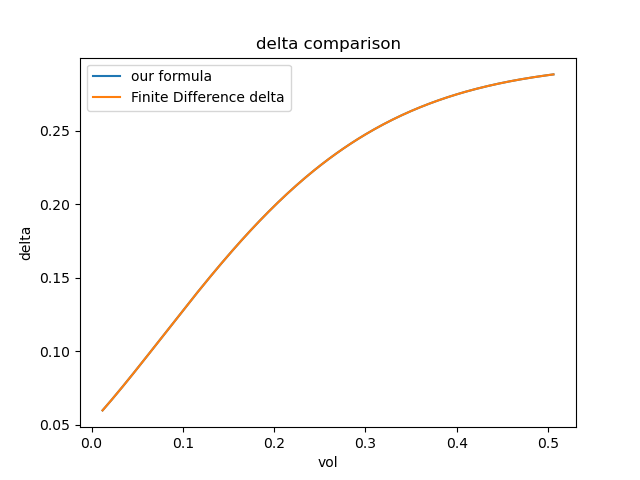
\includegraphics[width=0.5\textwidth]{./figures/delta comparison.png}\label{delta comparison}}
    \hfill
    \subfloat[absolute error between our formula and finite difference method]{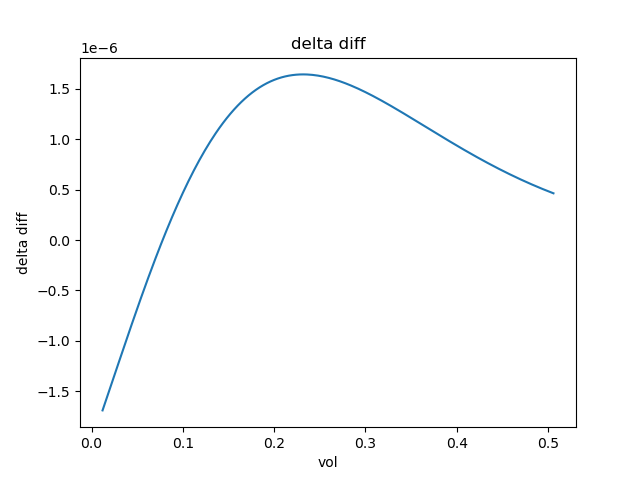
\includegraphics[width=0.5\textwidth]{./figures/delta diff.png}\label{delta diff}} \\
    \subfloat[Gamma comparison]{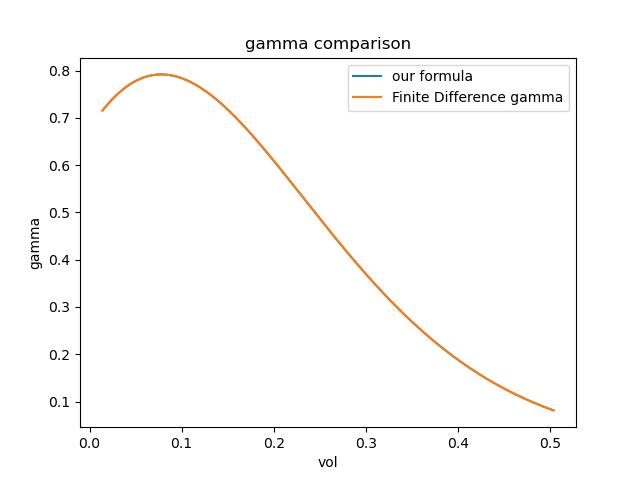
\includegraphics[width=0.5\textwidth]{./figures/gamma comparison.png}\label{gamma comparison}}
    \hfill
    \subfloat[absolute error between our formula and finite difference method]{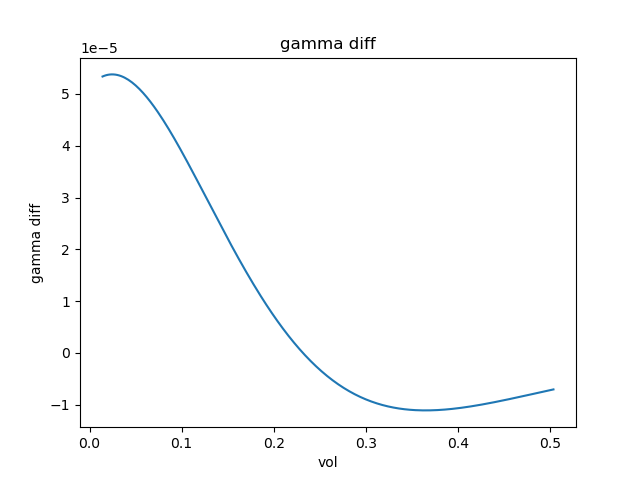
\includegraphics[width=0.5\textwidth]{./figures/gamma diff.png}\label{gamma diff}} \\
    \subfloat[Theta comparison]{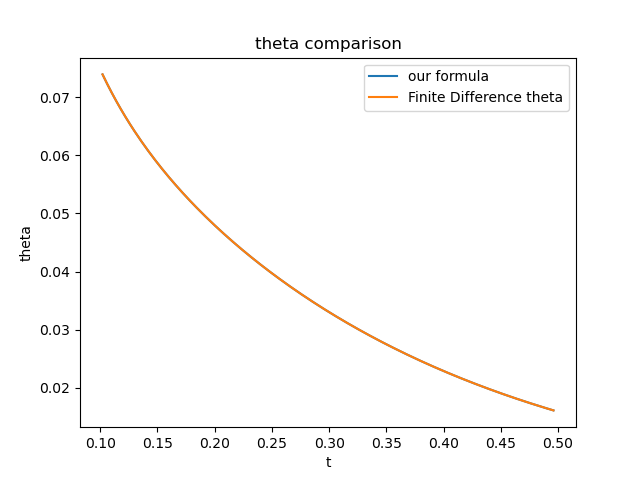
\includegraphics[width=0.5\textwidth]{./figures/theta comparison.png}\label{theta comparison}}
    \hfill
    \subfloat[absolute error between our formula and finite difference method]{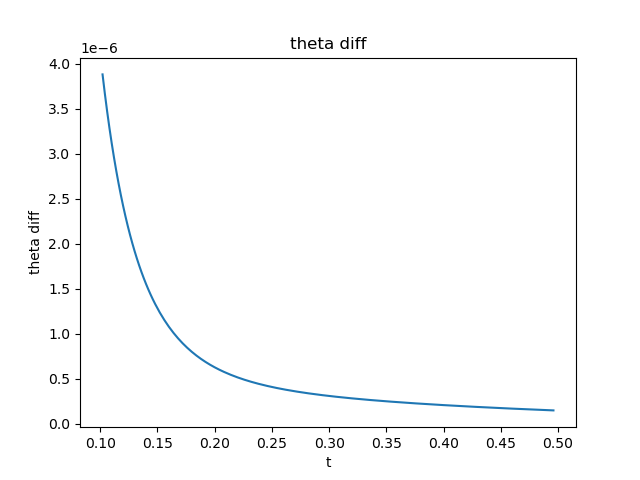
\includegraphics[width=0.5\textwidth]{./figures/theta diff.png}\label{theta diff}} 
    \caption{Three Greeks comparison between our formula and finite difference method}\label{greeks}
  \end{figure}

From \eqref{mispricing} we know that the mispricing function $\delta = \frac{1}{2} \sigma^2 (V^{2\gamma}-V) \Gamma_{\bar{w}}$, where $\Gamma_{\bar{w}}$ has been solved before. An attractive feature of Delta and Gamma is that they are sufficiently neat, making it easy for us to apply Ito-Taylor expansions on mispricing function later. Additionally, in essence, to apply Ito-Taylor expansions on mispricing function, we use the following algorithm as used in calculating delta and gamma:

\begin{enumerate}
    \item Use chain rule combining with \eqref{ccdf diff2} and \eqref{pdf diff2}to apply infinitesimal generator on current mispricing function $\delta_{n}$.
    \item Substitute PDFs inside $\delta_n$ with non-central parameter $\nu+i$ where $i \notin [2,6]$.
    \item Then we get $\delta_{n+1}$, to calculate higher order approximation formula, go back to step 1.
\end{enumerate}

Finally, we illustrate a method to implement KM's approximation method on volatility options under mean-reverting CEV model. Numerical results are shown in the next chapter.

\section{Approximating options under Heston plus CEV model}\label{sec: 3.2}

\cite{gatheral_consistent_2008} proposes volatility with double mean-reverting dynamics

$$
    \begin{aligned}
        d V_t &=\kappa_1 \left(V^{\prime}_t - V_t\right) d t+\sigma_{1} V^{\gamma_1}_t d W_t \\
        d V^{\prime}_t &=\kappa_2\left(\theta -V^{\prime}_t\right) d t+\sigma_{2} V^{\prime \gamma_2}_t d W^{\prime}_t
    \end{aligned}
$$

\noindent where $\gamma_1, \gamma_2 \in [\frac{1}{2},1]$, $dW_t dW^{\prime}_t = \rho dt$

\begin{itemize}
    \item It's called Double Heston model in the case $\gamma_1=\gamma_2=\frac{1}{2}$.
    \item The case $\gamma_1=\gamma_2=1$ Double Log-normal model.
    \item And the general Double CEV model.
\end{itemize}

We will discuss using our method to price options under double CEV model with $\gamma_1 = \frac{1}{2}, \gamma_2 \in [\frac{1}{2}, 1]$. We call it Heston plus CEV model. That is

$$
\begin{aligned}\label{heston cev}
    d V_t &=\kappa_1 \left(V^{\prime}_t - V_t\right) d t+\sigma_{1} \sqrt{V_t} d W_t \\
    d V^{\prime}_t &=\kappa_2\left(\theta -V^{\prime}_t\right) d t+\sigma_{2} V^{\prime \gamma}_t d W^{\prime}_t
\end{aligned}
$$

The same auxiliary model is used to price options, it's given by

$$
d V_t=\kappa(m - V_t) d t+\sigma \sqrt{V_t} d W_t
$$

\noindent Define infinitesimal generator $L$ for \eqref{heston cev} and $\bar{L}$ for SR mean-reverting model

\begin{equation}\label{inf gen2}
    \begin{aligned}
        L w=& \frac{\partial w}{\partial t}+\kappa_1(V^{\prime} - V) \frac{\partial w}{\partial V}+\frac{1}{2} \sigma_1^{2} V \frac{\partial^{2} w}{\partial V^{2}} \\
        &+ \kappa_2(\theta - V^{\prime}) \frac{\partial w}{V^{\prime}}+\frac{1}{2} \sigma_2^{2} V \frac{\partial^{2} w}{V^{\prime 2}} + \rho \sigma_1 \sigma_2 \sqrt{V} V^{\prime \gamma_2} \frac{\partial^2 w}{\partial V \partial V^{\prime}}\\
        \bar{L} w =& \frac{\partial w}{\partial t}+\kappa(m - V) \frac{\partial w}{\partial V}+\frac{1}{2} \sigma_1 V \frac{\partial^{2} w}{\partial V^{2}}
    \end{aligned}
\end{equation}

\noindent Mispricing function for it is then

$$
\begin{aligned}
    \delta = (L - \bar{L}) \bar{w} &= \kappa(V^{\prime}- m)\frac{\partial w}{\partial V} \\
    &= \kappa(V^{\prime}-m) \Delta{\bar{w}}
\end{aligned}
$$

\noindent where $\Delta{\bar{w}}$ is given in equation \eqref{delta}. We can use the same method illustrated in \ref{sec: 3.1} to apply Ito-Taylor expansions on it.